\documentclass[journal]{IEEEtran}

%%%% Using Latex Packages %%%%


\usepackage{cite}
\usepackage{amsmath,amssymb,amsfonts}
\usepackage{algorithmic}
\usepackage{subcaption}
\usepackage{color}
\usepackage{graphicx}
\usepackage{xcolor}
\usepackage{enumerate}
\usepackage{multirow}
\usepackage{amsmath}
\usepackage{amssymb}
\usepackage[utf8]{inputenc}
\usepackage[ruled]{algorithm2e}
\usepackage[colorinlistoftodos]{todonotes}
\def\BibTeX{{\rm B\kern-.05em{\sc i\kern-.025em b}\kern-.08em
    T\kern-.1667em\lower.7ex\hbox{E}\kern-.125emX}}
\newtheorem{definition}{Definition}
\renewcommand{\topfraction}{1.0}
\renewcommand{\bottomfraction}{1.0}
\renewcommand{\dbltopfraction}{1.0}
\renewcommand{\textfraction}{0.01}
\renewcommand{\floatpagefraction}{1.0}
\renewcommand{\dblfloatpagefraction}{1.0}
\setcounter{topnumber}{5}
\setcounter{bottomnumber}{5}
\setcounter{totalnumber}{10}


\hyphenation{op-tical net-works semi-conduc-tor}


\begin{document}

\title{Efficient Feasibility Checking Algorithm of Photovoltaic Array Reconfiguration}

\author{Dafang Zhao,
        Fukohito Ooshita,~\IEEEmembership{Member,~IEEE}
        and~Michiko~Inoue,~\IEEEmembership{Member,~IEEE}}% <-this % stops a space

% \thanks{M. Shell was with the Department
% of Electrical and Computer Engineering, Georgia Institute of Technology, Atlanta,
% GA, 30332 USA e-mail: (see http://www.michaelshell.org/contact.html).}% <-this % stops a space
% \thanks{J. Doe and J. Doe are with Anonymous University.}% <-this % stops a space
% \thanks{Manuscript received April 19, 2005; revised August 26, 2015.}}

% note the % following the last \IEEEmembership and also \thanks - 
% these prevent an unwanted space from occurring between the last author name
% and the end of the author line. i.e., if you had this:
% 
% \author{....lastname \thanks{...} \thanks{...} }
%                     ^------------^------------^----Do not want these spaces!


% make the title area
\maketitle

% As a general rule, do not put math, special symbols or citations
% in the abstract or keywords.
\begin{abstract}
  Power generation efficiency of photovoltaic (PV) systems is significantly affected buy partial shading and PV cell damage.
  Partial shading or PV cell damage induces mismatched power generation among PV panels.
  Conducted bypass diodes under mismatch conditions result in loss of efficiency in power generation.
  Mismatched PV array can be recovered by re-configuring electrical connections among PV panels in it.
  In this paper, a feasibility check problem of PV panel reconfiguration is introduced.
  This problem identifies whether a connection among PV panels can be configured from a given PV module level solution.
  Proposed algorithm evaluated by comparison with the exhaustive search through random shading distributed PV array.
  The experimental results demonstrate that proposed algorithm can identify feasible configurations more than 49,000 times faster than the exhaustive search with around 0.5\% errors.
\end{abstract}

% Note that keywords are not normally used for peerreview papers.
\begin{IEEEkeywords}
PV reconfiguration, partial-shading, mismatch, feasibility, heuristic
\end{IEEEkeywords}

\IEEEpeerreviewmaketitle



\section{Introduction}\label{sec:introduction}
\IEEEPARstart{I}{n} recent years, the use of green and renewable energy sources has been increased with the aim to reduce fossil fuel depletion and environment pollution.
Photovoltaic (PV) energy is one of the most promising emerging technologies.
PV market growth by improvements of converting unlimited solar energy into electrical energy as well as the cost reductions of PV panels.

The use of PV systems for power generation brings many challenges.
Due to the nature of PV cell, which is the basic component of PV array.
PV system easily suffers from various forms of system faults, which include physical damage, temperature in-homogeneity, or partial shading.
Unlike cell damage or other system faults, partial shading sources from cloud, dust or snow are very hard to prevent and predict.
Thus, when PV cell could not uniformly generate power when they experience different irradiance or been damaged.
This unbalanced working scenario will lead whole system mismatch.
Mismatch condition might accelerate heating or aging of PV cells and furthermore hinder operation of maximum power point tracking (MPPT) algorithm, especially when the PV array output P-V curve becomes non-convex\cite{islam2018performance}.

For several series connected PV cells, shaded or damaged cell causing normal cells to produce higher voltages that may reverse bias of ``bad'' cells.
When a large number of series connected cells cause a huge reverse bias across shaded cells, leading to large dissipation of energy in the ``bad'' cells.
This huge energy dissipation occurring in a small area might get overheating or burning of PV cells, or ``hot-spots''.
To protect PV cells from ``hot-spots'', bypass diode is used to circumvent concentrated energy dissipation.
However, the operation of bypass diode will cause several stop delivering power and generate multiple local maximum power points or the total PV module current are limited by the one of worst ``bad'' cell.
In both situation, available energy is lost.
Furthermore, strand bypass diode can not complete eliminate hot-spotting\cite{kim2015reexamination}.

In order to improve PV system power generation efficiency and protect PV cells from damage, an efficient and effectively PV system manage method is worth to investigate.
The key to improve power generation efficiency is to maintain maximum output power.
Thus, different maximum power point tracking (MPPT) algorithms have been proposed in this regard.
In different MPPT algorithms, P\&O\cite{kasa2000maximum,jain2004new,chomsuwan2002photovoltaic,wasynezuk1983dynamic}and hill climbing\cite{koutroulis2001development,teulings1993new,xiao2004modified} methods received many attention due to its low complexity and implement cost.
Hill climbing and P\&O methods are different ways to implement the same fundamental method.
Using the approximate linear relationship between $V_{OC}$,$I_{SC}$ and $V_{MPP}$, $I_{MPP}$, fractional voltage-based and current-based MPPT are popular due to their linear dependency of PV panel characteristic and irradiance level\cite{Liu2016,kobayashi2004novel,bekker2004finding,mutoh2002prediction,noguchi2001short}.
However, under abnormal working condition such as partial shading, it is very hard for conventional MPPT algorithms to find global maximum power point.
Meanwhile, without any PV module level improvement, it is impossible to protect PV panel against hot-spotting\cite{Olalla2018,ghanbari2016permanent}.

Another attractive direction to improve PV system efficiency under different working condition is the reconfiguration of PV arrays.
This concept was first proposed by Salameh $et$ $al.$\cite{Salameh1990} in 1990.
Then in 2002, Sherif and Boutros $et$ $al.$ proposed a reconfigurable scheme for PV arrays that using transistors as switch network to improve performance\cite{sherif2002solar}.
Nguyen $et$ $al.$ proposed a method that divide PV array into two parts as the ``fixed'' part which is static connected PV modules and ``adaptive'' part that can be attached to ``fixed'' part with different configurations\cite{Nguyen2008}.

In this type of ``fixed'' - ``adaptive'' architecture, the mathematical formulation is not clear.
Moreover, if the partial shading part is large enough to cover ``adaptive'' part, this scheme become ineffective.
Velasco $et$ $al.$\cite{Velasco-Quesada2009,velasco2008grid,velasco2005energy} proposed an principle of operation is referred as ``irradiance equalization''.
Reconfiguration strategy based on this principle aim to relocate the PV panels on the rows so that ``irradiance equalization'' is achieved.
However, optimal configuration requires differences between ``row'' irradiance level are minimized as shown in \cite{Velasco-Quesada2009} therefore it can only be realized on fully reconfigurable array.
They proposed algorithm that calculate all possible configurations and stored as look-up table locally.
Then, the ``best'' configuration for real-time shading scenario will be chosen from look-up table.
There is no doubt that the number of possible configurations will increase from the size of the PV array and it will be more difficult to determine the optimal configuration with limited time.
Though there are several reconfiguration methods have been proposed, most works consider reconfiguration in PV cell or PV module level.
However, those reconfiguration requires a significantly high computation time or a large number of switches to implement reconfiguration.
In addition, they require special PV panels with the capability of switching, and cannot be applied to the system constructed with standard PV panels.
Orozco-Gutierrez et al. proposed an efficient and effective reconfiguration method~\cite{Orozco-Gutierrez2016} where it first selects candidates of configurations using the product of approximated currents and voltages,
then finds the best one with precise power simulation. 
However, these candidates are specified in a PV module level though PV modules could not be fully reconfigured. Actually, we found that some of configuration candidates are not able to be realized. However, the paper~\cite{Orozco-Gutierrez2016}  does not show any systematic way to identify such a feasibility. 

This paper proposes an optimization algorithm to check possibilities of configurations for reconfiguring PV arrays, which uses an approach that limit and sort possible combinations by the index of ``Loss-rate''.
Proposed feasibility checking algorithm can rapidly check feasibility that a given configuration candidate can be actually formed by given PV panels.
The experimental results demonstrate the effectiveness of the proposed method where it can identify the feasibility of configurations with a very small false negative rate of less than 1\%.

\section{PV Array Reconfiguration}\label{sec:pv-array-reconf}
In this paper, we use following definition for PV array.
A PV array is formed by PV panels.
Several PV panels connected in series form a $String$.
A PV panel is formed by three series-connected PV modules.
A PV module consists of several series-connected PV cells with reverse biased bypass diode.
Figure~\ref{fig:array} represent the definition are introduced above.
\begin{figure}[ht]
\centerline{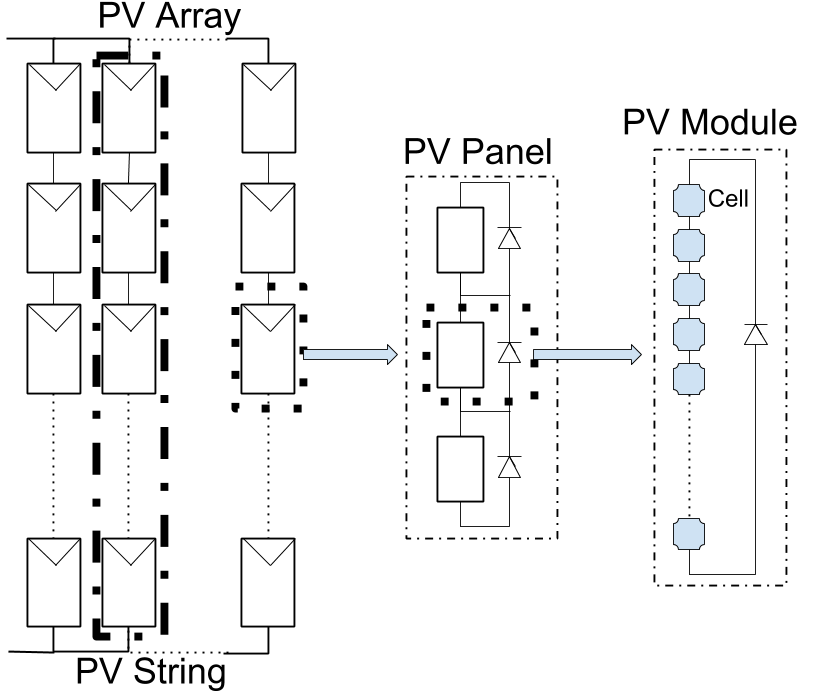
\includegraphics[width=\linewidth]{fig/module.png}}
\caption[]{PV array, string, module and panel}
\label{fig:array}
\end{figure}
In a PV array, we have two constraints.
PV panels in the same string have the same current level, while all the strings have the same control voltage.
When considering reconfiguration of PV panel, we should find out the best configuration while considering these constraints.

As addressed in section~\ref{sec:introduction}, Orozco-Guierrez et al. proposed an efficient reconfiguration algorithm for mismatched PV arrays.
The method utilizes information of MPPs of every PV panel that is extracted using an online monitoring\cite{Carotenuto2014} and a power estimation\cite{Orozco-Gutierrez2015}.

Firstly, maximum power points of PV panels are extracted by using online monitoring from\cite{Carotenuto2014}.
Then the current and voltage levels of maximum power point for each PV module $s$, $I_{mpp_{s}}$and $V_{mpp_{s}}$, are estimated from maximum power points of PV panels using the method in\cite{Orozco-Gutierrez2015}.

Estimated maximum power point current values ($I_{mpp_s}$) are approximated and close values are grouped into a small number of classes so that the number of possible combinations, in other words, search space is reduced.
Estimated maximum power point voltage values ($V_{mpp_s}$) are averaged and the mean value $\Bar{V}_{mpp}$ of all PV modules is used to approximate MPP voltage in the string.
MPP voltage is approximated by $m \times \Bar{V}_{mpp} $ where $m$ is the number of active modules at the MPP.
Then possible combination of configurations are enumerated.

For furthermore power simulation and configuration implementation, the current sequence and number of activating PV modules pre-string (it is called $feasibility$) are examined for each configuration.
A simple feasibility checking method provided in \cite{Orozco-Gutierrez2016} are described as follow.

\textbf{(Feasibility 1)}\footnote{In \cite{Orozco-Gutierrez2016}, only the case of $n=2$ is considered, and we extended the condition to general $n$. }
For each $n$-th highest current level $I_{n}$ in a current sequence $Q$ for strings,
it is required that the number of active modules in a configuration is $N(I_{n}) / n$ or less, where $N(I)$ is the total number of active modules for a current level $I$. 
The maximum number $M$ of active modules for a PV array is given as
\begin{equation}
    M=\mbox{min}\begin{Bmatrix}
N(I),\frac{N(I_2)}{2},\frac{N(I_3)}{3},\cdots,\frac{N(I_{n})}{n}
\end{Bmatrix}.
\label{eq:1}
\end{equation}
Thus, approximated power $P$ can be calculated as follow.
\begin{equation}
\label{eq:2}
P=\sum{Q}\times M \times \Bar{V}_{mpp}
\end{equation}

Approximated power values with and only with \textbf{Feasibility 1} is satisfied are listed into a power matrix like Table~\ref{tab:power-matrix}.
The configuration with  maximum power value and configurations whose powers are more than 77\% of maximum power are selected as configuration candidates\cite{Orozco-Gutierrez2016}.

\section{Feasibility}


\begin{table*}[t]
  \caption{}
  \centerline{APPROXIMATED POWER}
  \vskip5pt
\label{tab:power-matrix}
\centering
\begin{tabular}{c|rrrrrrrrrrr}
\hline\hline	
\# modules & 	\multicolumn{10}{c}{currents sequence for strings (A)} \\ 																
per string		&	\multicolumn{1}{c}{(3,3)}	&	\multicolumn{1}{c}{(3,2.5)}	&	\multicolumn{1}{c}{(3,1.5)}	&	\multicolumn{1}{c}{(3,0.5)}	&	\multicolumn{1}{c}{(2.5,2.5)}	&	\multicolumn{1}{c}{(2.5,1.5)}	&	\multicolumn{1}{c}{(2.5,0.5)}	&	\multicolumn{1}{c}{(1.5,1.5)}	&	\multicolumn{1}{c}{(1.5,0.5)}	&	\multicolumn{1}{c}{(0.5,0.5)}	\\ \hline
	1	&	120W	&	110W	&	90W	&	70W	&	100W	&	80W	&	60W	&	60W	&	40W	&	20W	\\ \hline
	2	&	-	&	220W	&	180W	&	140W	&	200W	&	160W	&	120W	&	120W	&	80W	&	40W	\\ \hline	3	&	-	&\textbf{330W}&	270W	&	210W	&	\textbf{300W}	&	240W	&	180W	&	180W	&	120W	&	60W	\\ \hline
4	&	-	&	-	&	-	&	-	&	-	&	\textbf{320W}	&	240W	&	240W	&	160W	&	80W	\\ \hline
	 5	&	-	&	-	&	-	&	-	&	-	&	-	&	\textbf{300W}	&	-	&	200W	&	100W	\\ \hline
	6	&	-	&	-	&	-	&	-	&	-	&	-	&	-	&	-	&	240W	&	120W	\\ \hline
\end{tabular}
\end{table*}

From Orozco $et$ $al.$ method, to complete reconfiguration, we need to assign panels into strings to realize a candidate configuration.
For example, consider a candidate configuration for a current sequence (2.5A, 2.5A) with 3 active modules per string as shown in Table~\ref{tab:power-matrix}
It can be realized by assigning panel P2 to the first string and panel P1 and P4 to the second string as shown in Figure~\ref{fig:feasibleassign}.
However, for another current sequence (2.5A, 1.5A), there is no feasible assignment for 4 active modules per string, even though this configuration is listed in Table~\ref{tab:power-matrix} by method in\cite{Orozco-Gutierrez2016}.
It is same for a configuration candidate with current sequence (3A, 2.5A) for 3 active modules per string.
That is, the condition \textbf{Feasibility 1} is necessary but not sufficient to give an actual feasibility result.

For a PV array $A$ with $s$ strings, let $M_{A,i}(I)$ denotes the number of modules that can be activated with a current level $I$ in the $i$-th string.
Let $Q = (Q_1,Q_2,\dots,Q_s)$ be the sequence of current required for strings.
We define the feasibility as follows: A sequence of current $Q$ is feasible with $m$ modules if and only if it is possible to form a PV array $A$ such that
\begin{equation}
  M_{A,i}(Q_i)\geq m
  \label{eq:3}
\end{equation}
holds for each string $i$ (1$\leq i \leq s$).

\begin{figure}[htbp]
    \centering
    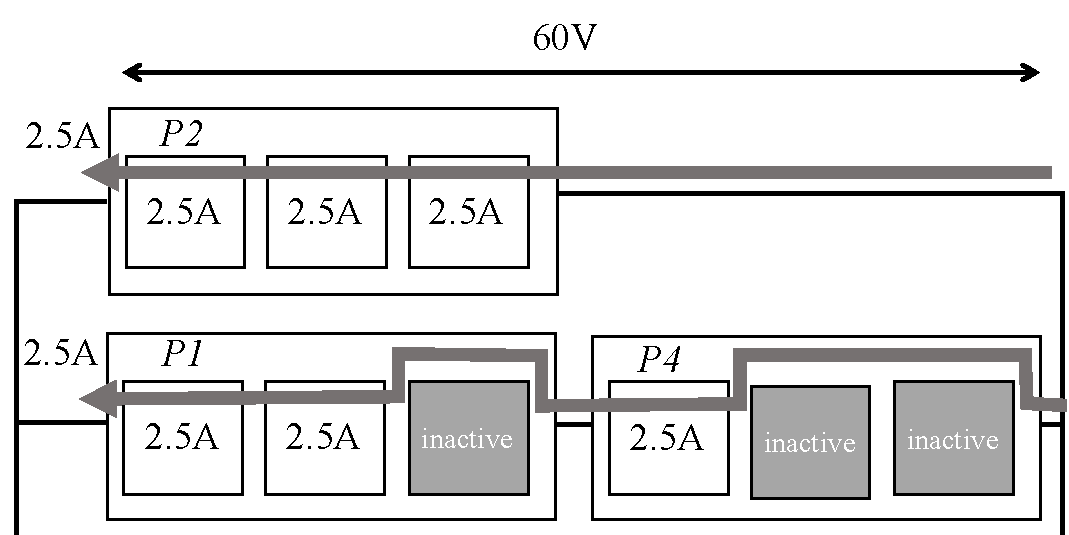
\includegraphics[width=\linewidth]{fig/feasible-configuration.pdf}
    \caption{Feasible configuration for a current sequence (2.5A, 2.5A) with 3 active modules.}
    \label{fig:feasibleassign}
\end{figure}

\section{Algorithm to identify feasibility}\label{sec:algor-ident-feas}
\subsection{Feasibility problem}\label{sec:feasibility-problem}
In this section, we introduce an algorithm to identify feasibility for a configuration.
First we will formulate the feasibility problem that identifies the feasibility for a given current sequence and the number of active modules per string as follows.

\textit{Definition 1} (\textit{Feasibility Problem}):\\
\textbf{Input}: Information of MPPs (approximated values), a current sequence $Q$, the number of $m$ of active modules per-string.\\
%\newline
\textbf{Output}: Whether $Q$ with $m$ modules is feasible or not.

\subsection{Outline of the algorithm}\label{sec:outline-algorithm}
\subsection{Algorithm}\label{sec:algorithm}
\section{Experiment Results}\label{sec:experiment-results}
\section{Conclusion}\label{sec:conclusion}
The conclusion goes here.



\appendices
\section*{Acknowledgment}


The authors would like to thank...


% Can use something like this to put references on a page
% by themselves when using endfloat and the captionsoff option.
% \section*{Temp}
% It is well known that mismatch due to partial shading, soiling, or ageing causes significant losses
% in the energy yield of photovoltaic (PV) systems [1,2]. Furthermore, mismatches may hinder operation
% of maximum power point (MPP) tracking algorithms, especially if the power versus output voltage
% characteristic becomes nonconvex [3]. It has also been shown that, even with commonly used bypass
% diodes, mismatched cells may become reverse-biased and dissipate power, producing an undesired
% cell temperature rise or hot spot [4,5]. This may lead to accelerated ageing and reduced reliability of
% the PV system


\bibliographystyle{ieeetr}
\bibliography{library}


\end{document}


